% Supplemental figures and tables (from EQCCTPro_Draft.md Material section)
\section*{Material}

The following pages contain \textbf{Tables 1--6} plus workflow diagrams (\textbf{Figures 1--3}) and enlarged rotated results figures (\textbf{Figures 4--8}).

\clearpage
\begin{figure}[H]
\centering
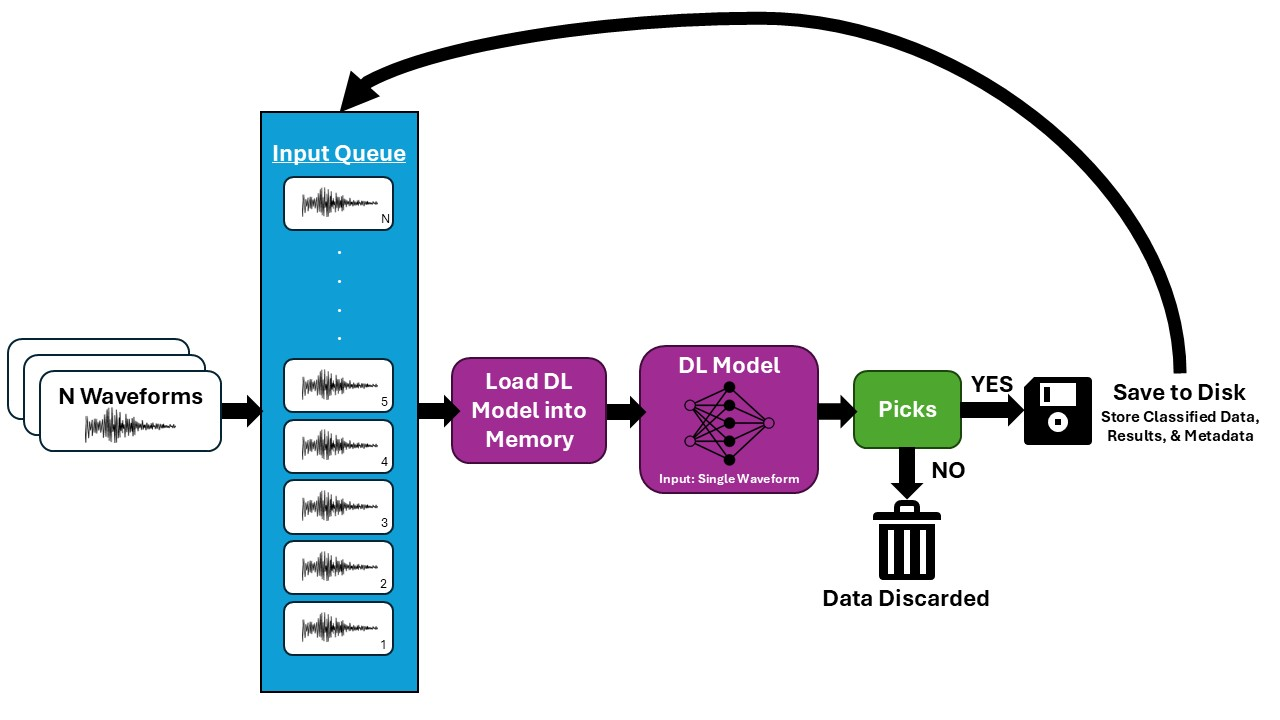
\includegraphics[width=0.92\linewidth]{figures/fig1.JPG}
\caption*{Figure 1. Serial baseline workflow. Waveforms are processed sequentially by a single DL model instance. Each waveform must wait for the previous one to complete, creating a linear bottleneck that scales poorly with network size.}
\end{figure}

\clearpage
\begin{figure}[H]
\centering
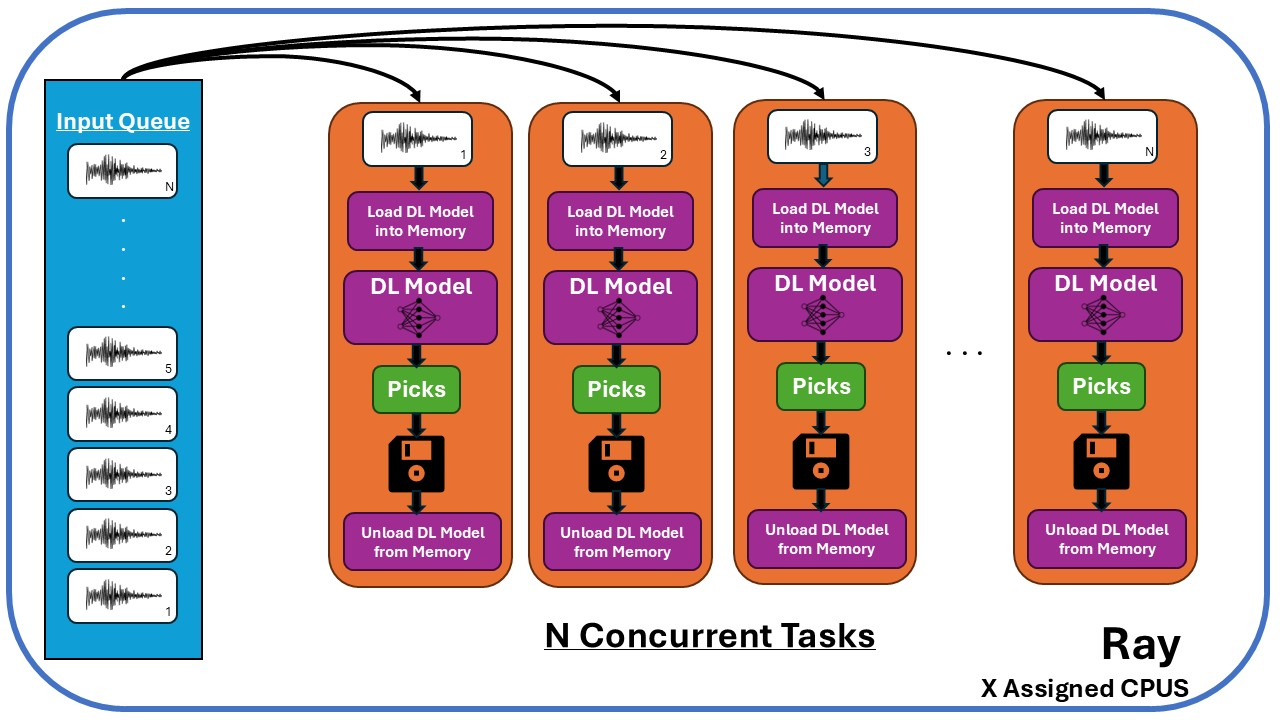
\includegraphics[width=0.92\linewidth]{figures/fig2.JPG}
\caption*{Figure 2. Ripper workflow. Each task independently loads the model, performs inference, and unloads. Multiple tasks run in parallel but incur repeated framework initialization overhead per station.}
\end{figure}

\clearpage
\begin{figure}[H]
\centering

\includegraphics[width=0.92\linewidth]{figures/fig3.PNG}
\caption*{Figure 3. Model-Actor workflow. Persistent inference actors maintain loaded models in memory (or GPU VRAM). Waveforms are dispatched to actors as a stream, eliminating load/unload overhead and maximizing throughput.}
\end{figure}

\clearpage
\begin{figure}[H]
\centering
\rotatebox{90}{%
  \begin{minipage}{0.85\textheight}
    \centering
    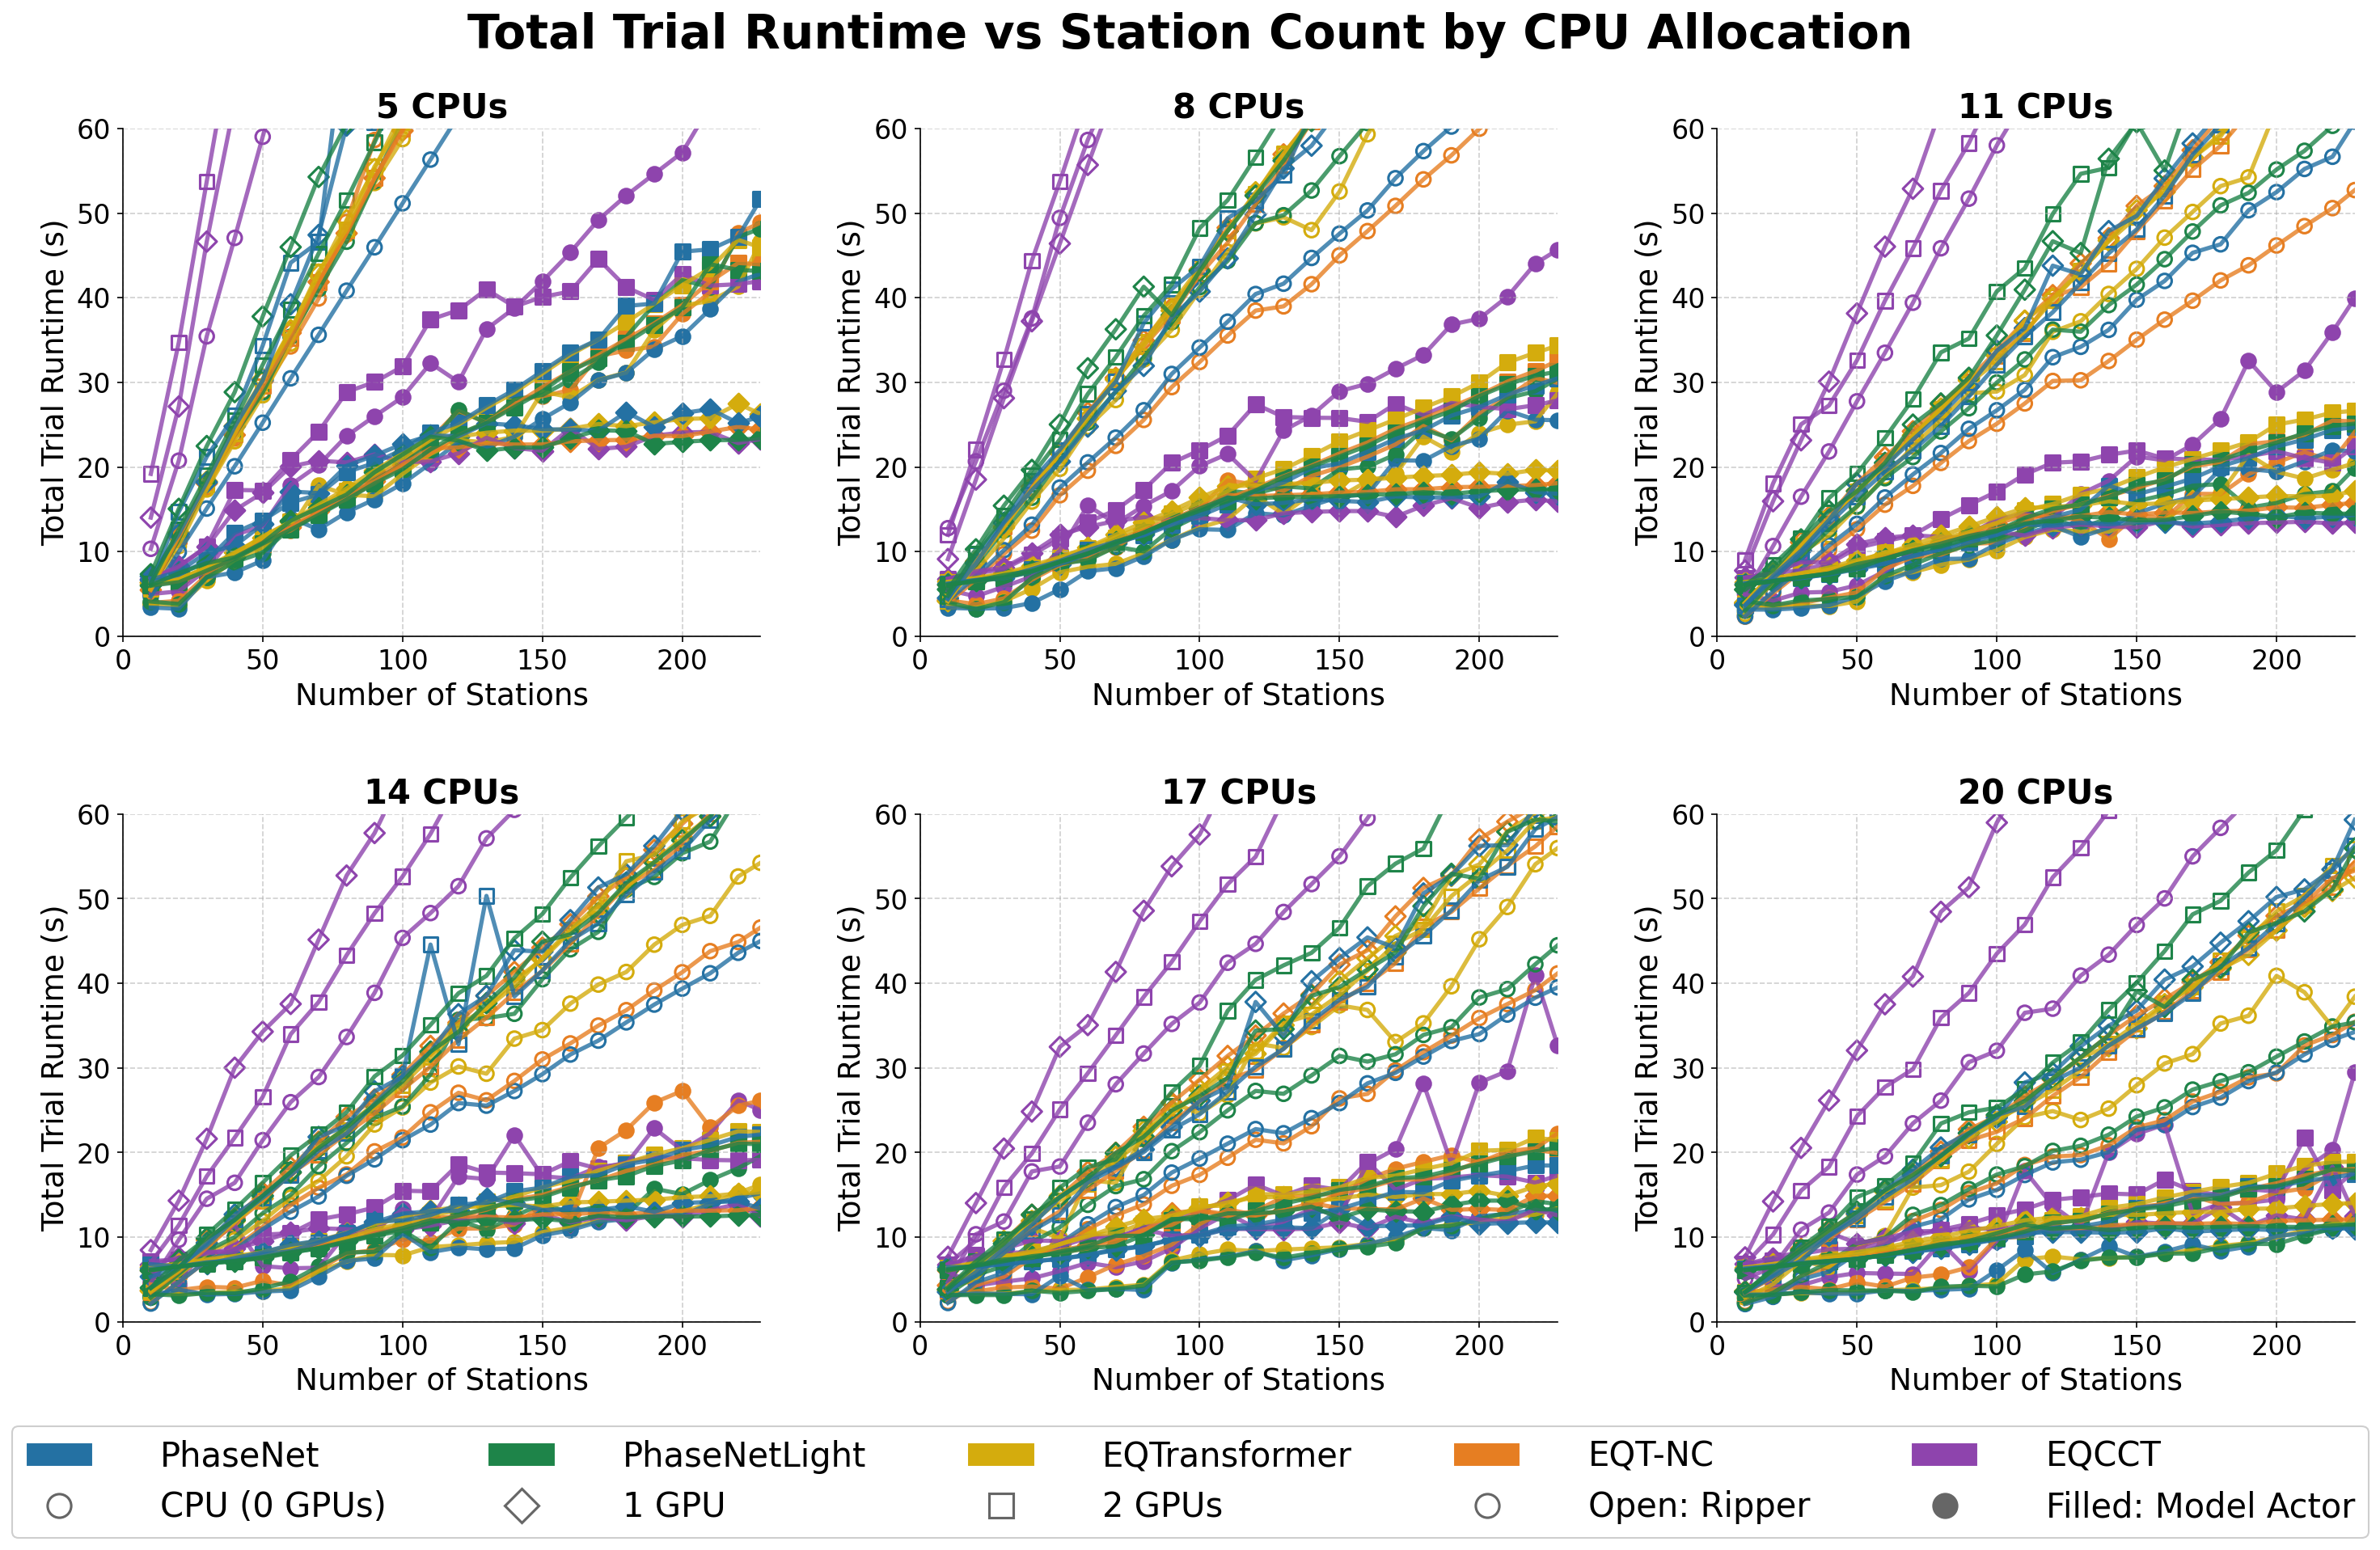
\includegraphics[width=\linewidth]{figures/fig4_runtime_3d.png}
    \caption*{Figure 4. Comparison of total trial runtime across all models and parallelization methods. Data points are plotted every 10 stations from 10 to 228. Fig.~5 and Table~4 summarize best 228-station totals.}
  \end{minipage}%
}
\end{figure}

\clearpage
\begin{figure}[H]
\centering
\rotatebox{90}{%
  \begin{minipage}{0.85\textheight}
    \centering
    
\includegraphics[width=\linewidth]{figures/fig5.png}
    \caption*{Figure 5. Minimum total runtime at 228 stations for Ripper versus Model-Actor (left: CPU, right: GPU). Bars are best successful end-to-end times at 228 stations per strategy. Dashed red line: 30~s target.}
  \end{minipage}%
}
\end{figure}

\clearpage
\begin{figure}[H]
\centering
\rotatebox{90}{%
  \begin{minipage}{0.85\textheight}
    \centering
    
\includegraphics[width=\linewidth]{figures/fig6.png}
    \caption*{Figure 6. Peak process-tree RAM (CPU) and VRAM (GPU) from the load-only benchmark: all $N$ workers held resident while sampling; bars show the maximum over 25~s samples (1.25~s interval). $N$ from best 228-station trial rows; R = Ripper tasks, MA = actors.}
  \end{minipage}%
}
\end{figure}

\clearpage
\begin{figure}[H]
\centering
\rotatebox{90}{%
  \begin{minipage}{0.85\textheight}
    \centering
    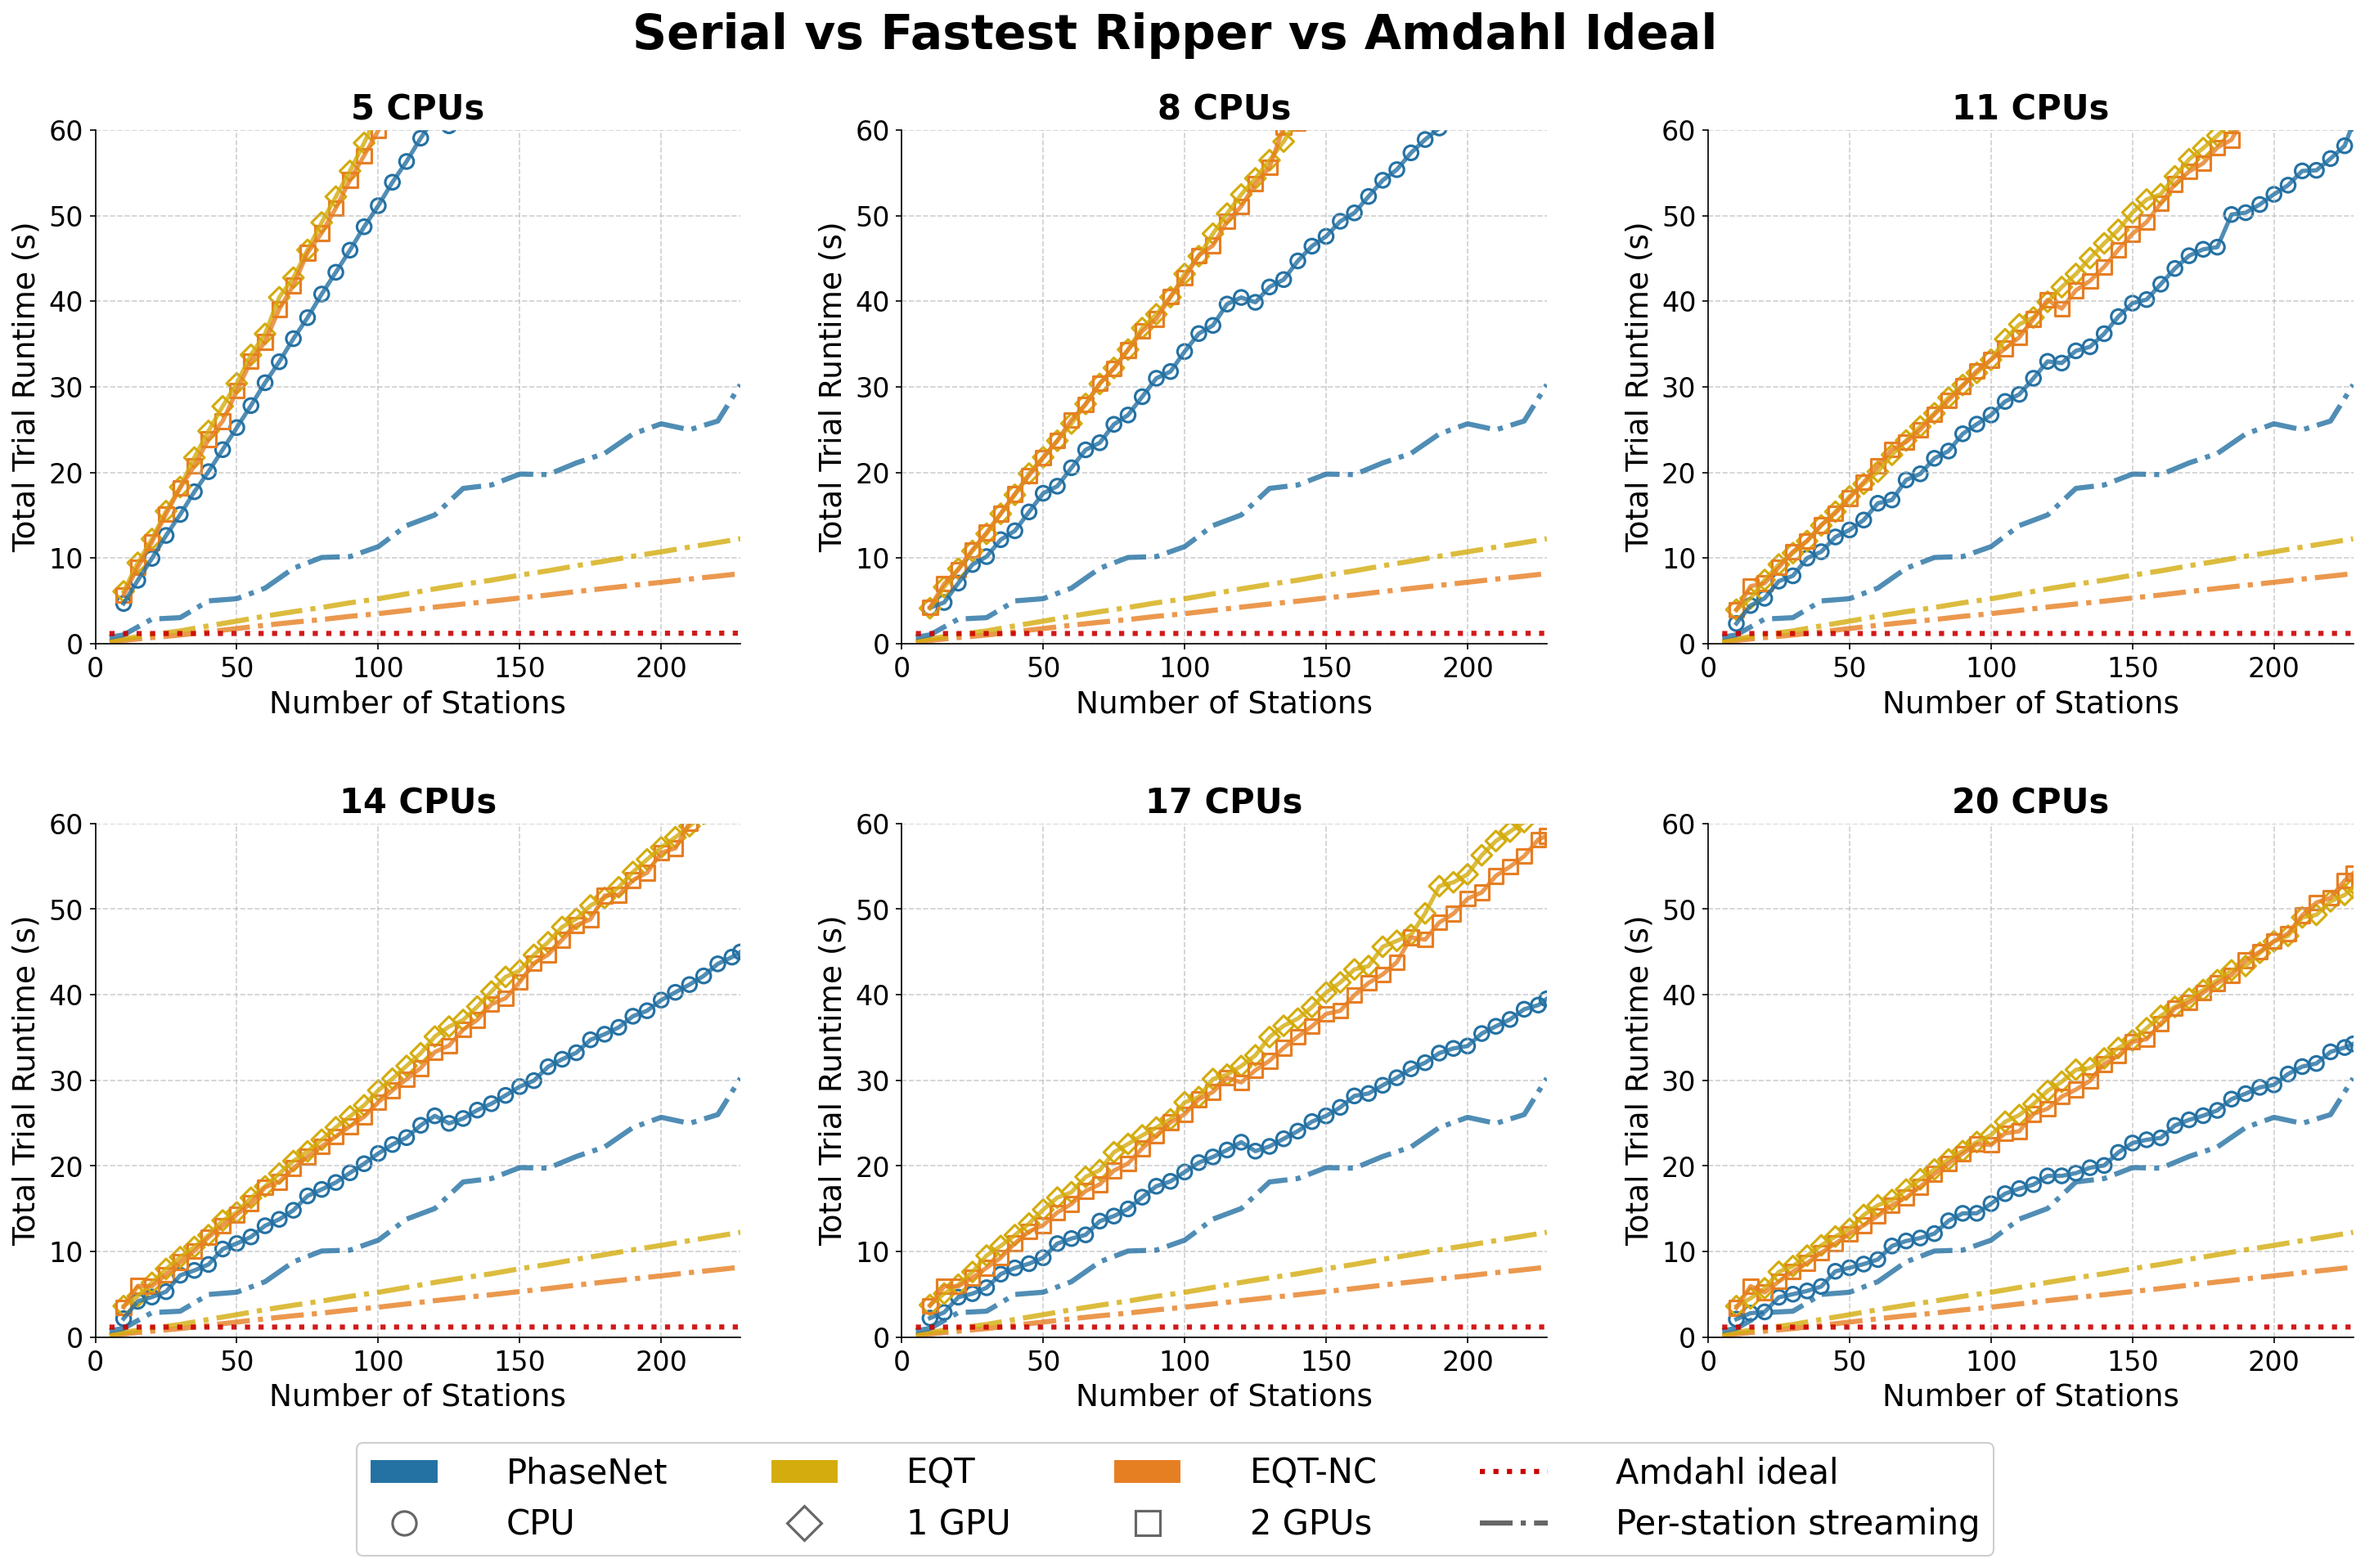
\includegraphics[width=\linewidth]{figures/fig7_serial_vs_ripper.png}
    \caption*{Figure 7. Serial baseline versus fastest Ripper configurations, with the batch-based Amdahl reference shown for each CPU allocation. For each Ripper hardware class, a single model is selected from the tested pool based on the lowest \emph{mean} total runtime across successful trials; this model defines the Ripper curve in each panel. Serial curves use the CPU spot-check grid in Table~2 (interpolated between anchors). The figure emphasizes scaling with network size rather than the individual minima reported in Table~4.}
  \end{minipage}%
}
\end{figure}

\clearpage
\begin{figure}[H]
\centering
\rotatebox{90}{%
  \begin{minipage}{0.85\textheight}
    \centering
    
\includegraphics[width=\linewidth]{figures/fig8_serial_vs_modelactor.png}
    \caption*{Figure 8. Serial baselines versus fastest Model-Actor configurations, with the Amdahl ideal limit shown for each CPU allocation. As in Figure 7, a single model is selected based on the lowest \emph{mean} total runtime across successful trials; this model defines the Model-Actor curve in each panel. Serial curves use the CPU spot-check grid in Table~2. The red dotted line denotes the Amdahl ideal, representing the theoretical minimum runtime under perfectly scalable batch processing.}
  \end{minipage}%
}
\end{figure}

\clearpage
\begin{landscape}

\begin{center}
\textbf{Table 1.} Single-process SeisBench baselines: load (minimum over five fresh load cycles), merged-stream \texttt{annotate()} on all \(N\) stations, and sequential \texttt{classify()} (mean wall time per station = total classify time divided by \(N\)). All times in seconds.

\vspace{0.8em}
\small
\begin{tabular}{lccccccc}
\toprule
\textbf{Model} & \textbf{Device} & \textbf{CPUs} & \textbf{GPUs} & \textbf{\(N\)} & \textbf{Load} & \textbf{Ann.} & \textbf{Cls./stn} \\
\midrule
PhaseNet       & CPU & 1 & 0 & 228 & 1.206 & 0.317 & 0.261 \\
PhaseNet       & GPU & 1 & 1 & 228 & 1.186 & 0.206 & 0.011 \\
PhaseNet       & CPU & 1 & 0 & 250 & 1.206 & 3.965 & 0.841 \\
PhaseNet       & GPU & 1 & 1 & 250 & 1.238 & 0.281 & 0.011 \\
PhaseNet       & CPU & 1 & 0 & 580 & 1.194 & 0.713 & 0.226 \\
PhaseNet       & GPU & 1 & 1 & 580 & 1.217 & 0.553 & 0.011 \\
PhaseNetLight  & CPU & 1 & 0 & 228 & 1.185 & 0.267 & 0.015 \\
PhaseNetLight  & GPU & 1 & 1 & 228 & 1.178 & 0.199 & 0.006 \\
PhaseNetLight  & CPU & 1 & 0 & 250 & 1.198 & 3.121 & 0.009 \\
PhaseNetLight  & GPU & 1 & 1 & 250 & 1.198 & 0.222 & 0.006 \\
PhaseNetLight  & CPU & 1 & 0 & 580 & 1.163 & 0.649 & 0.009 \\
PhaseNetLight  & GPU & 1 & 1 & 580 & 1.169 & 0.539 & 0.006 \\
EQTransformer  & CPU & 1 & 0 & 228 & 1.182 & 1.219 & 0.070 \\
EQTransformer  & GPU & 1 & 1 & 228 & 1.185 & 0.550 & 0.056 \\
EQTransformer  & CPU & 1 & 0 & 250 & 1.211 & 24.307 & 0.080 \\
EQTransformer  & GPU & 1 & 1 & 250 & 1.180 & 0.536 & 0.055 \\
EQTransformer  & CPU & 1 & 0 & 580 & 1.179 & 1.634 & 0.079 \\
EQTransformer  & GPU & 1 & 1 & 580 & 1.193 & 0.881 & 0.056 \\
EQT-NC         & CPU & 1 & 0 & 228 & 1.184 & 1.054 & 0.045 \\
EQT-NC         & GPU & 1 & 1 & 228 & 1.181 & 0.494 & 0.031 \\
EQT-NC         & CPU & 1 & 0 & 250 & 1.181 & 1.180 & 0.047 \\
EQT-NC         & GPU & 1 & 1 & 250 & 1.186 & 0.487 & 0.031 \\
EQT-NC         & CPU & 1 & 0 & 580 & 1.184 & 1.458 & 0.051 \\
EQT-NC         & GPU & 1 & 1 & 580 & 1.178 & 0.816 & 0.031 \\
\bottomrule
\end{tabular}
\end{center}

\end{landscape}

\clearpage
\begin{landscape}

\begin{center}
\textbf{Table 2.} CPU serial spot-checks (minimum over five runs per quantity). \textbf{Ann} = merged-stream \texttt{annotate()} time for all \(N\) stations; \textbf{Cls} = total sequential \texttt{classify()} time for all \(N\) stations (seconds). Load = minimum over five independent load cycles. Panel (a): TexNet 230-station subtree; (b): 250-station tree; (c): 580-station tree. These grids anchor the empirical serial curves in Figures~7--8.

\vspace{0.6em}
\scriptsize
\textbf{(a) \(N\) from 230-station dataset.}

\begin{tabular}{l r rrrrrrrrrrrr}
\toprule
\textbf{Model} & \textbf{Ld} & \multicolumn{2}{c}{\(N{=}10\)} & \multicolumn{2}{c}{\(N{=}50\)} & \multicolumn{2}{c}{\(N{=}100\)} & \multicolumn{2}{c}{\(N{=}150\)} & \multicolumn{2}{c}{\(N{=}200\)} & \multicolumn{2}{c}{\(N{=}228\)} \\
 & & Ann & Cls & Ann & Cls & Ann & Cls & Ann & Cls & Ann & Cls & Ann & Cls \\
\midrule
PhaseNet & 1.169 & 0.023 & 0.819 & 0.085 & 5.914 & 0.147 & 11.454 & 0.212 & 17.279 & 0.287 & 19.912 & 0.324 & 27.623 \\
PhaseNetLight & 1.169 & 0.020 & 0.064 & 0.068 & 0.326 & 0.143 & 0.652 & 0.185 & 0.973 & 0.229 & 1.306 & 0.265 & 1.481 \\
EQTransformer & 1.163 & 0.087 & 0.585 & 0.206 & 2.762 & 0.471 & 5.496 & 0.672 & 8.305 & 0.879 & 11.003 & 1.016 & 12.541 \\
EQT-NC & 1.163 & 0.069 & 0.386 & 0.186 & 1.796 & 0.432 & 3.568 & 0.660 & 5.437 & 0.884 & 7.302 & 1.011 & 8.302 \\
\bottomrule
\end{tabular}

\vspace{1em}
\textbf{(b) \(N\) from 250-station dataset.}

\begin{tabular}{l r rrrrrrrrrrrrr}
\toprule
\textbf{Model} & \textbf{Ld} & \multicolumn{2}{c}{\(N{=}10\)} & \multicolumn{2}{c}{\(N{=}50\)} & \multicolumn{2}{c}{\(N{=}100\)} & \multicolumn{2}{c}{\(N{=}150\)} & \multicolumn{2}{c}{\(N{=}200\)} & \multicolumn{2}{c}{\(N{=}228\)} & \multicolumn{2}{c}{\(N{=}250\)} \\
 & & Ann & Cls & Ann & Cls & Ann & Cls & Ann & Cls & Ann & Cls & Ann & Cls & Ann & Cls \\
\midrule
PhaseNet & 1.175 & 0.019 & 1.125 & 0.066 & 6.108 & 0.142 & 12.321 & 0.194 & 18.014 & 0.244 & 24.590 & 0.289 & 25.883 & 0.324 & 31.498 \\
PhaseNetLight & 1.181 & 0.017 & 0.064 & 0.061 & 0.323 & 0.125 & 0.650 & 0.170 & 0.975 & 0.226 & 1.294 & 0.262 & 1.477 & 0.290 & 1.619 \\
EQTransformer & 1.178 & 0.080 & 0.581 & 0.158 & 2.609 & 0.371 & 5.410 & 0.631 & 8.188 & 0.779 & 10.955 & 0.960 & 12.528 & 1.014 & 13.740 \\
EQT-NC & 1.157 & 0.059 & 0.384 & 0.137 & 1.746 & 0.348 & 3.611 & 0.606 & 5.441 & 0.821 & 7.298 & 0.912 & 8.342 & 1.011 & 9.151 \\
\bottomrule
\end{tabular}

\vspace{1em}
\textbf{(c) \(N\) from 580-station dataset.}

\begin{tabular}{l r rrrrrrrrrrrrrrr}
\toprule
\textbf{Model} & \textbf{Ld} & \multicolumn{2}{c}{\(N{=}10\)} & \multicolumn{2}{c}{\(N{=}50\)} & \multicolumn{2}{c}{\(N{=}100\)} & \multicolumn{2}{c}{\(N{=}150\)} & \multicolumn{2}{c}{\(N{=}200\)} & \multicolumn{2}{c}{\(N{=}228\)} & \multicolumn{2}{c}{\(N{=}250\)} & \multicolumn{2}{c}{\(N{=}580\)} \\
 & & Ann & Cls & Ann & Cls & Ann & Cls & Ann & Cls & Ann & Cls & Ann & Cls & Ann & Cls & Ann & Cls \\
\midrule
PhaseNet & 1.158 & 0.020 & 0.797 & 0.063 & 5.738 & 0.114 & 11.293 & 0.163 & 17.230 & 0.228 & 22.941 & 0.266 & 27.778 & 0.283 & 30.640 & 0.634 & 67.109 \\
PhaseNetLight & 1.165 & 0.018 & 0.063 & 0.059 & 0.319 & 0.108 & 0.637 & 0.153 & 0.963 & 0.214 & 1.287 & 0.243 & 1.461 & 0.265 & 1.600 & 0.589 & 3.736 \\
EQTransformer & 1.143 & 0.075 & 0.595 & 0.155 & 2.872 & 0.213 & 5.493 & 0.302 & 9.314 & 0.432 & 11.276 & 0.481 & 12.696 & 0.518 & 13.912 & 1.316 & 32.663 \\
EQT-NC & 1.171 & 0.057 & 0.379 & 0.117 & 1.886 & 0.189 & 3.503 & 0.288 & 5.479 & 0.410 & 7.382 & 0.483 & 8.291 & 0.479 & 9.111 & 1.274 & 21.449 \\
\bottomrule
\end{tabular}
\end{center}

\end{landscape}

\clearpage
\begin{landscape}

\begin{center}
\textbf{Table 3.} Per-instance memory budgets (MB) used by RAPID to cap concurrency and avoid out-of-memory errors.

\vspace{1em}
\small
\begin{tabular}{llccccccc}
\toprule
\textbf{Model} & \textbf{Framework} & \multicolumn{2}{c}{\textbf{Host RAM -- CPU (MB)}} & \multicolumn{2}{c}{\textbf{Host RAM -- GPU (MB)}} & \multicolumn{3}{c}{\textbf{GPU VRAM (MB)}} \\
\cmidrule(lr){3-4} \cmidrule(lr){5-6} \cmidrule(lr){7-9}
 & & Base & Per Ripper/Actor & Base & Per Ripper/Actor & Base & Per Ripper & Per Actor \\
\midrule
PhaseNet      & PyTorch    & 502  & 2,038 & 870  & 2,406 & 500  & 850  & 1,524 \\
PhaseNetLight & PyTorch    & 502  & 2,038 & 861  & 2,397 & 500  & 850  & 1,524 \\
EQTransformer & PyTorch    & 521  & 2,057 & 1,001 & 2,537 & 528  & 1,056 & 1,552 \\
EQT-NC        & PyTorch    & 524  & 2,060 & 1,017 & 2,553 & 530  & 1,060 & 1,554 \\
EQCCT         & TensorFlow & 728  & 2,264 & 2,311 & 3,847 & 1,732 & 3,464 & 2,756 \\
\bottomrule
\end{tabular}
\end{center}

\end{landscape}

\clearpage
\begin{landscape}

\begin{center}
\textbf{Table 4.} Best successful Ripper total time at 228 stations, sorted by fastest time. CPU rows are minima over Ray CPUs tested; GPU rows report the best one-GPU and two-GPU Ripper totals separately.

\vspace{0.8em}
\small
\begin{tabular}{lccccc}
\toprule
\textbf{Model} & \textbf{Device} & \textbf{CPUs} & \textbf{GPUs} & \textbf{Conc. Tasks} & \textbf{Ripper Picking/Total (s)} \\
\midrule
PhaseNet         & CPU & 20 & 0 & 91  & 34.25 \\
PhaseNetLight    & CPU & 20 & 0 & 91  & 35.38 \\
EQTransformer-NC & CPU & 20 & 0 & 228 & 35.45 \\
EQTransformer    & CPU & 20 & 0 & 137 & 38.42 \\
EQTransformer    & GPU & 20 & 1 & 22  & 52.48 \\
EQTransformer-NC & GPU & 20 & 1 & 22  & 53.31 \\
EQTransformer-NC & GPU & 20 & 2 & 44  & 54.17 \\
EQTransformer    & GPU & 20 & 2 & 44  & 55.88 \\
PhaseNetLight    & GPU & 20 & 1 & 22  & 55.95 \\
PhaseNet         & GPU & 20 & 2 & 44  & 56.27 \\
PhaseNet         & GPU & 20 & 1 & 22  & 59.32 \\
PhaseNetLight    & GPU & 20 & 2 & 44  & 67.61 \\
EQCCT            & CPU & 20 & 0 & 137 & 76.07 \\
EQCCT            & GPU & 20 & 2 & 24  & 96.10 \\
EQCCT            & GPU & 20 & 1 & 12  & 127.35 \\
\bottomrule
\end{tabular}
\end{center}

\end{landscape}

\clearpage
\begin{landscape}

\begin{center}
\textbf{Table 5.} Best successful Model-Actor total time at 228 stations, sorted by fastest time. CPU rows are minima over Ray CPUs tested; GPU rows report the best one-GPU and two-GPU Model-Actor totals separately. Setup OH is actor-creation (or equivalent) setup time as a percentage of total Model-Actor trial time.

\vspace{1em}
\small
\begin{tabular}{lcccccccc}
\toprule
\textbf{Model} & \textbf{Device} & \textbf{CPUs} & \textbf{GPUs} & \textbf{Actors} & \textbf{Setup (s)} & \textbf{Pick (s)} & \textbf{Total (s)} & \textbf{Setup OH} \\
\midrule
PhaseNet      & GPU & 20 & 1 & 22 & 6.70  & 4.27 & 10.97 & 61.0\% \\
PhaseNetLight & CPU & 20 & 0 & 46 & 7.04  & 4.28 & 11.47 & 61.4\% \\
PhaseNet      & CPU & 20 & 0 & 46 & 7.21  & 4.16 & 11.48 & 62.8\% \\
PhaseNetLight & GPU & 20 & 1 & 22 & 6.96  & 4.56 & 11.53 & 60.4\% \\
EQTransformer & CPU & 20 & 0 & 46 & 6.92  & 4.70 & 11.63 & 59.5\% \\
EQT-NC        & GPU & 20 & 1 & 22 & 6.91  & 5.19 & 12.11 & 57.1\% \\
EQCCT         & GPU & 14 & 1 & 12 & 4.64  & 7.82 & 12.47 & 37.2\% \\
EQTransformer & GPU & 20 & 1 & 22 & 7.12  & 6.92 & 14.05 & 50.7\% \\
EQCCT         & GPU & 17 & 2 & 24 & 7.95  & 9.33 & 17.29 & 46.0\% \\
PhaseNet      & GPU & 20 & 2 & 44 & 10.88 & 6.60 & 17.49 & 62.2\% \\
EQT-NC        & CPU & 20 & 0 & 46 & 12.88 & 4.70 & 17.74 & 72.6\% \\
PhaseNetLight & GPU & 20 & 2 & 44 & 10.83 & 7.02 & 17.86 & 60.6\% \\
EQT-NC        & GPU & 20 & 2 & 44 & 10.75 & 7.30 & 18.06 & 59.5\% \\
EQTransformer & GPU & 20 & 2 & 44 & 10.76 & 8.16 & 18.93 & 56.9\% \\
EQCCT         & CPU & 14 & 0 & 46 & 12.73 & 12.23 & 25.01 & 50.9\% \\
\bottomrule
\end{tabular}
\end{center}

\end{landscape}

\clearpage
\begin{landscape}

\begin{center}
\textbf{Table 6.} Memory utilization for each Model-Actor row in Table~5. All memory values are in MB.

\vspace{1em}
\small
\begin{tabular}{lccccccccc}
\toprule
\textbf{Model} & \textbf{Device} & \textbf{CPUs} & \textbf{GPUs} & \textbf{Actors} & \textbf{Req. RAM} & \textbf{Tree RAM} & \textbf{Req. VRAM} & \textbf{Tree VRAM} & \textbf{Peak RAM} \\
\midrule
PhaseNet      & GPU & 20 & 1 & 22 & 58,564  & 32,813 & 36,344 & 11,580 & 782 \\
PhaseNetLight & CPU & 20 & 0 & 46 & 105,524 & 49,017 & 0      & 0      & 273 \\
PhaseNet      & CPU & 20 & 0 & 46 & 105,524 & 51,694 & 0      & 0      & 274 \\
PhaseNetLight & GPU & 20 & 1 & 22 & 58,366  & 39,068 & 36,344 & 11,580 & 280 \\
EQTransformer & CPU & 20 & 0 & 46 & 106,398 & 51,012 & 0      & 0      & 258 \\
EQT-NC        & GPU & 20 & 1 & 22 & 61,798  & 43,578 & 37,004 & 12,273 & 244 \\
EQCCT         & GPU & 14 & 1 & 12 & 49,236  & 15,363 & 34,608 & 40,316 & 456 \\
EQTransformer & GPU & 20 & 1 & 22 & 61,446  & 42,982 & 36,960 & 12,226 & 275 \\
EQCCT         & GPU & 17 & 2 & 24 & 98,472  & 18,506 & 69,216 & 43,675 & 958 \\
PhaseNet      & GPU & 20 & 2 & 44 & 117,128 & 59,490 & 72,688 & 526    & 1,084 \\
EQT-NC        & CPU & 20 & 0 & 46 & 106,536 & 56,537 & 0      & 0      & 200 \\
PhaseNetLight & GPU & 20 & 2 & 44 & 116,732 & 72,936 & 72,688 & 23,161 & 383 \\
EQT-NC        & GPU & 20 & 2 & 44 & 123,596 & 82,457 & 74,008 & 24,545 & 378 \\
EQTransformer & GPU & 20 & 2 & 44 & 122,892 & 80,613 & 73,920 & 24,453 & 398 \\
EQCCT         & CPU & 14 & 0 & 46 & 115,920 & 48,701 & 0      & 0      & 202 \\
\bottomrule
\end{tabular}
\end{center}

\end{landscape}
